% Created 2022-10-10 Mon 10:56
% Intended LaTeX compiler: pdflatex
\documentclass[10pt]{beamer}
\usepackage[utf8]{inputenc}
\usepackage[T1]{fontenc}
\usepackage{graphicx}
\usepackage{longtable}
\usepackage{wrapfig}
\usepackage{rotating}
\usepackage[normalem]{ulem}
\usepackage{amsmath}
\usepackage{amssymb}
\usepackage{capt-of}
\usepackage{hyperref}
\usepackage{minted}
\usepackage{xcolor}
\definecolor{LightGray}{gray}{0.95}
\usefonttheme{professionalfonts}
\setlength{\parskip}{5pt}
\newcommand{\footnoteframe}[1]{\footnote[frame]{#1}}
\addtobeamertemplate{footnote}{}{\vspace{2ex}}
\usepackage{tabularx}
\usepackage{booktabs}
\DefineVerbatimEnvironment{verbatim}{Verbatim}{fontsize=\scriptsize}
\usetheme{Berkeley}
\author{Jay Morgan}
\date{21st September 2022}
\title{Programming Level-up}
\subtitle{Lecture 4 -- An Introduction to Numerical Computing in Python}
\hypersetup{
 pdfauthor={Jay Morgan},
 pdftitle={Programming Level-up},
 pdfkeywords={},
 pdfsubject={},
 pdfcreator={Emacs 27.1 (Org mode 9.4.6)}, 
 pdflang={English}}
\begin{document}

\maketitle
\begin{frame}{Outline}
\tableofcontents
\end{frame}


\section{NumPy}
\label{sec:orga0fe9eb}

\subsection{What is NumPy}
\label{sec:orga11af75}

\begin{frame}[label={sec:org012091d},fragile]{What is NumPy?}
 NumPy (\url{https://numpy.org/}) is one of the fundamental Python libraries for scientific
computing. In essence, its aim is to make vector and array processing in Python much
more efficient. Therefore, it would be your go-to for (numerical) data
processing.

Numerical data processing with NumPy can, most often that not, be magnitudes faster
than what you can write in Python, even if the operations are the same. This is
because NumPy is partly written in C.

For example, if we want to compute the matrix multiplication of two arrays:

\begin{minted}[frame=lines,linenos=true,firstnumber=last,fontsize=\footnotesize,bgcolor=LightGray,xleftmargin=5pt,tabsize=2,breaklines=true,numbersep=10pt]{python}
A = [[1, 4], [9, 5]]  # 2 dimensional 'matrices' A and B
B = [[1, 2], [3, 4]]
C = [[0, 0], [0, 0]]  # our result 'pre-allocated' with zeros

for i in range(len(A)):
    for j in range(len(B)):
        for k in range(len(B)):
            C[i][j] += A[i][k] * B[k][j]
\end{minted}
\end{frame}

\begin{frame}[label={sec:orgbde2806},fragile]{What is NumPy?}
 The previous example is quite un-weidly. We have to manually loop through the
matrices and apply the computation for each element. This can be \alert{very} slow in
Python. NumPy provides a much cleaner and quicker interface:

\begin{minted}[frame=lines,linenos=true,firstnumber=last,fontsize=\footnotesize,bgcolor=LightGray,xleftmargin=5pt,tabsize=2,breaklines=true,numbersep=10pt]{python}
import numpy as np
A = np.array([[1, 4], [9, 5]])
B = np.array([[1, 2], [3, 4]])
C = A @ B  # or np.matmul(A, B)
print(C)
\end{minted}

\begin{verbatim}
Results: 
# => [[13 18]
# =>  [24 38]]
\end{verbatim}
\end{frame}

\begin{frame}[label={sec:orgccaec42},fragile]{Install NumPy}
 Before we can use NumPy, we must first install it if its not already. NumPy can
easily be installed with one of your package managers of choice. For example, if you
want to install via conda:

\begin{minted}[frame=lines,linenos=true,firstnumber=last,fontsize=\footnotesize,bgcolor=LightGray,xleftmargin=5pt,tabsize=2,breaklines=true,numbersep=10pt]{bash}
conda install numpy
\end{minted}

or with pip:

\begin{minted}[frame=lines,linenos=true,firstnumber=last,fontsize=\footnotesize,bgcolor=LightGray,xleftmargin=5pt,tabsize=2,breaklines=true,numbersep=10pt]{bash}
pip install numpy
\end{minted}
\end{frame}

\begin{frame}[label={sec:orgf3df2bc},fragile]{Creating a numpy array}
 As we've seen previously, we use \texttt{np.array} to create a numpy array from a Python data type

\begin{minted}[frame=lines,linenos=true,firstnumber=last,fontsize=\footnotesize,bgcolor=LightGray,xleftmargin=5pt,tabsize=2,breaklines=true,numbersep=10pt]{python}
A = np.array([[1, 2, 3], [4, 5, 6], [7, 8, 9]])
print(A)
\end{minted}

\begin{verbatim}
Results: 
# => [[1 2 3]
# =>  [4 5 6]
# =>  [7 8 9]]
\end{verbatim}


We've created a 3x3 matrix of integers. Note that, out-of-the-box, NumPy doesn't
support \emph{ragged arrays} (matrices that are not rectangular), so this will not work as
you expect:

\begin{minted}[frame=lines,linenos=true,firstnumber=last,fontsize=\footnotesize,bgcolor=LightGray,xleftmargin=5pt,tabsize=2,breaklines=true,numbersep=10pt]{python}
A = np.array([[1], [1, 2]])
\end{minted}
\end{frame}

\subsection{Working with NumPy}
\label{sec:orga2c45b6}

\begin{frame}[label={sec:org75dc59f},fragile]{Basic attributes}
 A numpy array has various attributes that are useful for our numerical
computing. Some of these include:

\begin{minted}[frame=lines,linenos=true,firstnumber=last,fontsize=\footnotesize,bgcolor=LightGray,xleftmargin=5pt,tabsize=2,breaklines=true,numbersep=10pt]{python}
A = np.array([[1, 4], [9, 5]])

print(A.shape)  # the shape of the array
print(A.size)   # number of elements
print(A.ndim)   # number of dimensions
print(A.nbytes) # storage used
print(A.dtype)  # data type of elements
\end{minted}

\begin{verbatim}
Results: 
# => (2, 2)
# => 4
# => 2
# => 32
# => int64
\end{verbatim}
\end{frame}

\begin{frame}[label={sec:orge775d6b},fragile]{Different data types}
 In the previous example, the elements in the array we \texttt{int64}. But normally, we will
see \texttt{float64}. However, there are many other available data types, where each of the
different data types affects how much memory is used to represent the data.

\begin{itemize}
\item int (8, 16, 32, 64)
\item uint (unsigned integers)
\item bool
\item float (8, 16, 32, 64)
\item complex
\end{itemize}

\url{https://numpy.org/doc/stable/user/basics.types.html}
\url{https://numpy.org/doc/stable/reference/arrays.dtypes.html}
\end{frame}

\begin{frame}[label={sec:orgd8ef56b},fragile]{Creating arrays with different dtypes}
 When creating a NumPy array, NumPy will select what it thinks to be the most
appropriate data type. However, we can tell NumPy explicitly what the data type
should be with the \texttt{dtype} argument.

\begin{minted}[frame=lines,linenos=true,firstnumber=last,fontsize=\footnotesize,bgcolor=LightGray,xleftmargin=5pt,tabsize=2,breaklines=true,numbersep=10pt]{python}
A = np.array([[1, 2], [9, 5]], dtype=np.int8)
print(A)
print(A.dtype)

A = np.array([[1, 2], [9, 5]], dtype=np.float)
print(A)
print(A.dtype)
\end{minted}

\begin{verbatim}
Results: 
# => [[1 2]
# =>  [9 5]]
# => int8
# => [[1. 2.]
# =>  [9. 5.]]
# => float64
\end{verbatim}
\end{frame}

\begin{frame}[label={sec:org43ac423},fragile]{Changing dtypes}
 In some cases, we wish to change the data type of arrays \emph{after} its creation. For this
we use the \texttt{.astype()} method. This method takes a single argument: the data type you
wish to change the array to.

\begin{minted}[frame=lines,linenos=true,firstnumber=last,fontsize=\footnotesize,bgcolor=LightGray,xleftmargin=5pt,tabsize=2,breaklines=true,numbersep=10pt]{python}
A = np.array([1, 2, 3, 4])
print(A.dtype)
\end{minted}

\begin{verbatim}
int64
\end{verbatim}


We could change it to a \texttt{float64} array:

\begin{minted}[frame=lines,linenos=true,firstnumber=last,fontsize=\footnotesize,bgcolor=LightGray,xleftmargin=5pt,tabsize=2,breaklines=true,numbersep=10pt]{python}
A = A.astype(float)
print(A.dtype)
\end{minted}

\begin{verbatim}
float64
\end{verbatim}


Or \texttt{float32}:

\begin{minted}[frame=lines,linenos=true,firstnumber=last,fontsize=\footnotesize,bgcolor=LightGray,xleftmargin=5pt,tabsize=2,breaklines=true,numbersep=10pt]{python}
A = A.astype(np.float32)
print(A.dtype)
\end{minted}

\begin{verbatim}
float32
\end{verbatim}
\end{frame}

\begin{frame}[label={sec:org4871d79},fragile]{Different ways of creating arrays}
 NumPy also provides us with a number of different functions to create arrays. Instead
of doing this:

\begin{minted}[frame=lines,linenos=true,firstnumber=last,fontsize=\footnotesize,bgcolor=LightGray,xleftmargin=5pt,tabsize=2,breaklines=true,numbersep=10pt]{python}
A = np.array([[0, 0], [0, 0]])
\end{minted}

We could instead use the \texttt{np.zeros} function, passing a tuple where each element of
the tuple describes how many elements should be made in each dimension:

\begin{minted}[frame=lines,linenos=true,firstnumber=last,fontsize=\footnotesize,bgcolor=LightGray,xleftmargin=5pt,tabsize=2,breaklines=true,numbersep=10pt]{python}
A = np.zeros((2,)) # 1 dimensional
A = np.zeros((2, 2))  # 2 dimensional
A = np.zeros((2, 5, 5))  # 3 dimensional
\end{minted}
\end{frame}

\begin{frame}[label={sec:org24843ee},fragile]{Different ways of creating arrays}
 Another commonly used array creation function is the \texttt{np.random.randn} function. This
creates an array where elements are sampled from a normal distribution.

\begin{minted}[frame=lines,linenos=true,firstnumber=last,fontsize=\footnotesize,bgcolor=LightGray,xleftmargin=5pt,tabsize=2,breaklines=true,numbersep=10pt]{python}
A = np.random.randn(2, 2)
print(A)
\end{minted}

\begin{verbatim}
Results: 
# => [[-0.68213848 -0.44274759]
# =>  [ 0.6748596   0.64244208]]
\end{verbatim}


\alert{Note} the interface is a little different than \texttt{.zeros}, where instead of passing a
tuple, we pass multiple arguments to the function.
\end{frame}

\begin{frame}[label={sec:orgab83b23},fragile]{Different ways of creating arrays}
 It is also convenient to create arrays with ranges of elements.

\begin{minted}[frame=lines,linenos=true,firstnumber=last,fontsize=\footnotesize,bgcolor=LightGray,xleftmargin=5pt,tabsize=2,breaklines=true,numbersep=10pt]{python}
A = np.arange(5, 10) # optional step
print(A)
\end{minted}

\begin{verbatim}
Results: 
# => [5 6 7 8 9]
\end{verbatim}


\begin{minted}[frame=lines,linenos=true,firstnumber=last,fontsize=\footnotesize,bgcolor=LightGray,xleftmargin=5pt,tabsize=2,breaklines=true,numbersep=10pt]{python}
A = np.linspace(5, 10, 20)
print(A)
\end{minted}

\begin{verbatim}
Results: 
# => [ 5.          5.26315789  5.52631579  5.78947368  6.05263158  6.31578947
# =>   6.57894737  6.84210526  7.10526316  7.36842105  7.63157895  7.89473684
# =>   8.15789474  8.42105263  8.68421053  8.94736842  9.21052632  9.47368421
# =>   9.73684211 10.        ]
\end{verbatim}
\end{frame}


\begin{frame}[label={sec:org99a7fac},fragile]{Different ways of creating arrays}
 There are many more ways to create arrays. Some include:

\begin{itemize}
\item \texttt{np.ones}  - a matrix of 1's
\item \texttt{np.eye} - an identity matrix
\item \texttt{np.diag} - create a matrix with supplied elements across the diagonal
\item \texttt{np.fromfunction} - load elements from the return of a function
\item \texttt{np.fromfile} - load elements from a data file
\end{itemize}

Though, the best resource for understanding is NumPy's own documentation on the
subject: \url{https://numpy.org/doc/stable/user/basics.creation.html}
\end{frame}

\subsection{Indexing Arrays}
\label{sec:orgbfa62a3}

\begin{frame}[label={sec:orgf1b9bc9},fragile]{Slicing NumPy arrays}
 In native Python, when we have a 'matrix' like data structure (just a list of lists),
and we want to access a particular element from this matrix, we have to do something
like:

\begin{minted}[frame=lines,linenos=true,firstnumber=last,fontsize=\footnotesize,bgcolor=LightGray,xleftmargin=5pt,tabsize=2,breaklines=true,numbersep=10pt]{python}
A = [[1, 2], [3, 4]]
print(A[1][0])
\end{minted}

\begin{verbatim}
Results: 
# => 3
\end{verbatim}


However, in NumPy, we seperate the indexes by comma:

\begin{minted}[frame=lines,linenos=true,firstnumber=last,fontsize=\footnotesize,bgcolor=LightGray,xleftmargin=5pt,tabsize=2,breaklines=true,numbersep=10pt]{python}
A = np.array([[1, 2], [3, 4]])
print(A[1, 0])
\end{minted}

\begin{verbatim}
Results: 
# => 3
\end{verbatim}
\end{frame}

\begin{frame}[label={sec:org3c9f6ce},fragile]{Slicing NumPy Arrays}
 If we wanted to get all elements from the 2nd column we would use the \texttt{:} notation. For
example:

\begin{minted}[frame=lines,linenos=true,firstnumber=last,fontsize=\footnotesize,bgcolor=LightGray,xleftmargin=5pt,tabsize=2,breaklines=true,numbersep=10pt]{python}
A = np.array([[1, 2], [3, 4]])
print(A[:, 1])
\end{minted}

\begin{verbatim}
Results: 
# => [2 4]
\end{verbatim}


Likewise, all elements from the 2nd row:

\begin{minted}[frame=lines,linenos=true,firstnumber=last,fontsize=\footnotesize,bgcolor=LightGray,xleftmargin=5pt,tabsize=2,breaklines=true,numbersep=10pt]{python}
print(A[1, :])
\end{minted}

\begin{verbatim}
Results: 
# => [3 4]
\end{verbatim}
\end{frame}

\begin{frame}[label={sec:org6224b95},fragile]{Slicing NumPy Arrays}
 Note that when we slice an array, we are \alert{not copying} the elements:

\begin{minted}[frame=lines,linenos=true,firstnumber=last,fontsize=\footnotesize,bgcolor=LightGray,xleftmargin=5pt,tabsize=2,breaklines=true,numbersep=10pt]{python}
A = np.array([[1, 2], [3, 4]])
b = A[:, 1]

b[0] = 10

print(A)
\end{minted}

\begin{verbatim}
Results: 
# => [[ 1 10]
# =>  [ 3  4]]
\end{verbatim}


Any modification you make to the \texttt{b} variable will also affect \texttt{A}. For that we must use
\texttt{.copy()}

\begin{minted}[frame=lines,linenos=true,firstnumber=last,fontsize=\footnotesize,bgcolor=LightGray,xleftmargin=5pt,tabsize=2,breaklines=true,numbersep=10pt]{python}
A = np.array([[1, 2], [3, 4]])
b = A[:, 1].copy()
...
\end{minted}
\end{frame}

\begin{frame}[label={sec:org882a33d},fragile]{Slicing NumPy Arrays}
 If we have a multi-dimensional array, to which we wish to index on the final
dimension, one way to achieve this is by doing the following:

\begin{minted}[frame=lines,linenos=true,firstnumber=last,fontsize=\footnotesize,bgcolor=LightGray,xleftmargin=5pt,tabsize=2,breaklines=true,numbersep=10pt]{python}
A = np.random.randn(10, 2, 5, 4)  # our array to slice
A[:, :, :, 1:2]  # slice on the last dimension
\end{minted}

This can get pretty tedious the more that the number of dimensions increases. But! we
have one syntactical shortcut at our disposal: the ellipses '\ldots{}'. Using the ellipses
in place of the many ':' slices on each dimension, we're telling NumPy to just take
all elements from the prior dimensions. For example:

\begin{minted}[frame=lines,linenos=true,firstnumber=last,fontsize=\footnotesize,bgcolor=LightGray,xleftmargin=5pt,tabsize=2,breaklines=true,numbersep=10pt]{python}
A[..., 1:2]  # same slice on the last dimension
\end{minted}
\end{frame}

\begin{frame}[label={sec:org7ecac6f}]{Slicing NumPy Arrays}
\begin{figure}[htbp]
\centering
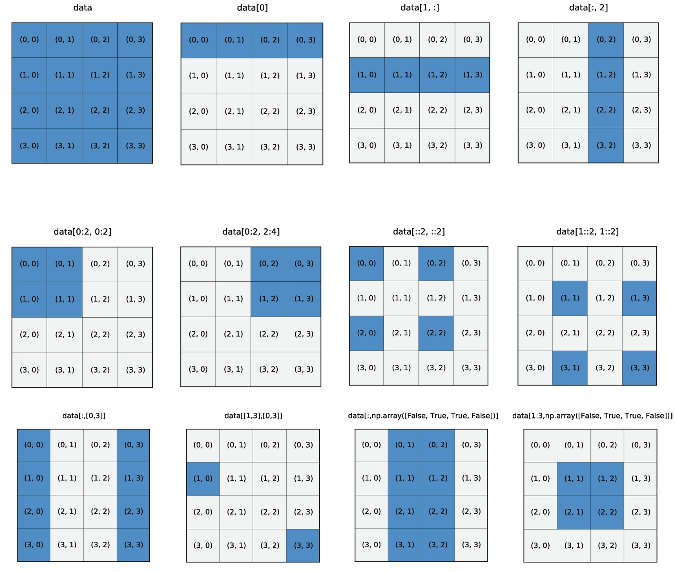
\includegraphics[width=0.7\textwidth]{./images/indexing.png}
\caption{Johansson, R., Johansson, R., \& John, S. (2019). Numerical Python (Vol. 1). Apress.P}
\end{figure}
\end{frame}

\begin{frame}[label={sec:orgdf02ac8},fragile]{Boolean Indexing}
 NumPy arrays can also be composed of boolean elements

\begin{minted}[frame=lines,linenos=true,firstnumber=last,fontsize=\footnotesize,bgcolor=LightGray,xleftmargin=5pt,tabsize=2,breaklines=true,numbersep=10pt]{python}
A = np.array([[1, -1], [0, 5]])
print(A > 0)
\end{minted}

\begin{verbatim}
Results: 
# => [[ True False]
# =>  [False  True]]
\end{verbatim}


And we can also use boolean elements to help with indexing:

\begin{minted}[frame=lines,linenos=true,firstnumber=last,fontsize=\footnotesize,bgcolor=LightGray,xleftmargin=5pt,tabsize=2,breaklines=true,numbersep=10pt]{python}
values_above_zero = A[A > 0]
print(values_above_zero)
\end{minted}

\begin{verbatim}
Results: 
# => [1 5]
\end{verbatim}
\end{frame}

\begin{frame}[label={sec:org324c02a},fragile]{Boolean Indexing}
 Therefore we can apply computations to only part of the array using this indexing
feature:

\begin{minted}[frame=lines,linenos=true,firstnumber=last,fontsize=\footnotesize,bgcolor=LightGray,xleftmargin=5pt,tabsize=2,breaklines=true,numbersep=10pt]{python}
mask = A > 0
A[mask] = A[mask] + 10
print(A)
\end{minted}

\begin{verbatim}
Results: 
# => [[11 -1]
# =>  [ 0 15]]
\end{verbatim}
\end{frame}

\subsection{Reshaping and Resizing}
\label{sec:org5a5de95}

\begin{frame}[label={sec:org81185ae},fragile]{Reshape}
 After an array has been created, we can modify its structure/shape using various
functions. The first we shall look at is \texttt{.reshape}. For example, let us create a
vector of 4 elements and then reshape it into an array of 2x2 elements. Of course,
the new shape of the array must be proportional to the original number of elements:
2x2 elements = 4 elements.

\begin{minted}[frame=lines,linenos=true,firstnumber=last,fontsize=\footnotesize,bgcolor=LightGray,xleftmargin=5pt,tabsize=2,breaklines=true,numbersep=10pt]{python}
A = np.arange(1, 5)

mat_A = A.reshape(2, 2)
print(mat_A)
print(A)  # A is not changed! No need for copy
\end{minted}

\begin{verbatim}
Results: 
# => [[1 2]
# =>  [3 4]]
# => [1 2 3 4]
\end{verbatim}
\end{frame}

\begin{frame}[label={sec:org85ab33a},fragile]{Flatten}
 If we wanted to take a 2d array and reshape it into a vector, we could of course use
the \texttt{.reshape} function again. But we could also use \texttt{.flatten}.

\begin{minted}[frame=lines,linenos=true,firstnumber=last,fontsize=\footnotesize,bgcolor=LightGray,xleftmargin=5pt,tabsize=2,breaklines=true,numbersep=10pt]{python}
flat_A = mat_A.flatten()
print(flat_A)
\end{minted}

\begin{verbatim}
Results: 
# => [1 2 3 4]
\end{verbatim}
\end{frame}

\begin{frame}[label={sec:org59b742b},fragile]{Flatten}
 When specifying the new dimensionality of the reshaped array, \texttt{-1} is a shortcut to
specify the dimensionality to allow reshaping to occur correctly. For example:

\begin{minted}[frame=lines,linenos=true,firstnumber=last,fontsize=\footnotesize,bgcolor=LightGray,xleftmargin=5pt,tabsize=2,breaklines=true,numbersep=10pt]{python}
A = np.arange(1, 5)
print(A)

print(A.reshape(2, -1))
\end{minted}

\begin{verbatim}
Results: 
# => [1 2 3 4]
# => [[1 2]
# =>  [3 4]]
\end{verbatim}


We're telling NumPy to create an array with 2 elements on the 1st dimension, and then
however many elements on the second dimension.
\end{frame}

\begin{frame}[label={sec:org602ab22},fragile]{Add a dimension}
 We can add and remove dimensions using \texttt{.expand\_dims} and \texttt{.squeeze}, respectively.

\begin{minted}[frame=lines,linenos=true,firstnumber=last,fontsize=\footnotesize,bgcolor=LightGray,xleftmargin=5pt,tabsize=2,breaklines=true,numbersep=10pt]{python}
print(A)
print(np.expand_dims(A, 1))
\end{minted}

\begin{verbatim}
Results: 
# => [1 2 3 4]
# => [[1]
# =>  [2]
# =>  [3]
# =>  [4]]
\end{verbatim}


We are taking a vector and adding a dimension. Note that we have to use
\texttt{np.expand\_dims} passing the object we want to expand and not \texttt{A.expand\_dims}.
\end{frame}

\begin{frame}[label={sec:org615d2b9},fragile]{Add a dimension}
 We can use an indexing trick with \texttt{None} to do the expansion in just the same way:

\begin{minted}[frame=lines,linenos=true,firstnumber=last,fontsize=\footnotesize,bgcolor=LightGray,xleftmargin=5pt,tabsize=2,breaklines=true,numbersep=10pt]{python}
print(A)
print(A[:, None])
\end{minted}

\begin{verbatim}
Results: 
# => [1 2 3 4]
# => [[1]
# =>  [2]
# =>  [3]
# =>  [4]]
\end{verbatim}


Where \texttt{None} indicates to NumPy where we want to add the new dimension.
\end{frame}

\begin{frame}[label={sec:org2a5ff6d},fragile]{Remove a dimension}
 If we want to instead remove a dimension, we can use \texttt{.squeeze()}

\begin{minted}[frame=lines,linenos=true,firstnumber=last,fontsize=\footnotesize,bgcolor=LightGray,xleftmargin=5pt,tabsize=2,breaklines=true,numbersep=10pt]{python}
print(A[:, None].squeeze(1))
\end{minted}

\begin{verbatim}
Results: 
# => [1 2 3 4]
\end{verbatim}


We are removing the 2nd dimension, but \alert{note} that the elements must be singletons. So
you cannot squeeze a 2x2 array.
\end{frame}

\begin{frame}[label={sec:org3ab4fc5},fragile]{Matrix transpose}
 Another useful feature is the matrix transpose:

\begin{minted}[frame=lines,linenos=true,firstnumber=last,fontsize=\footnotesize,bgcolor=LightGray,xleftmargin=5pt,tabsize=2,breaklines=true,numbersep=10pt]{python}
print(mat_A)

print(mat_A.transpose())
\end{minted}

\begin{verbatim}
Results: 
# => [[1 2]
# =>  [3 4]]
# => [[1 3]
# =>  [2 4]]
\end{verbatim}


or even:

\begin{minted}[frame=lines,linenos=true,firstnumber=last,fontsize=\footnotesize,bgcolor=LightGray,xleftmargin=5pt,tabsize=2,breaklines=true,numbersep=10pt]{python}
print(mat_A.T)
\end{minted}

\begin{verbatim}
Results: 
# => [[1 3]
# =>  [2 4]]
\end{verbatim}
\end{frame}


\begin{frame}[label={sec:orgb3e169c},fragile]{Composing arrays}
 If we have multiple arrays we want to 'join' together, we can use \texttt{np.hstack} for
horizontally joining, or \texttt{np.vstack} for vertically joining arrays. \alert{Note} the dimensions
must match in the direction your stacking.

\begin{minted}[frame=lines,linenos=true,firstnumber=last,fontsize=\footnotesize,bgcolor=LightGray,xleftmargin=5pt,tabsize=2,breaklines=true,numbersep=10pt]{python}
A = np.array([1, 2, 3])
B = np.array([4, 5, 6])

print(np.hstack([A, B]))
\end{minted}

\begin{verbatim}
[1 2 3 4 5 6]
\end{verbatim}


\begin{minted}[frame=lines,linenos=true,firstnumber=last,fontsize=\footnotesize,bgcolor=LightGray,xleftmargin=5pt,tabsize=2,breaklines=true,numbersep=10pt]{python}
print(np.vstack([A, B]))
\end{minted}

\begin{verbatim}
Results: 
# => [[1 2 3]
# =>  [4 5 6]]
\end{verbatim}
\end{frame}

\begin{frame}[label={sec:org5012433},fragile]{Composing arrays using concatenate}
 \texttt{hstack} and \texttt{vstack} can be useful when the required output shape is simply
defined. However, there is a more general function - \texttt{np.concatenate} - that will be
more often useful to us.

\begin{minted}[frame=lines,linenos=true,firstnumber=last,fontsize=\footnotesize,bgcolor=LightGray,xleftmargin=5pt,tabsize=2,breaklines=true,numbersep=10pt]{python}
print(np.concatenate([A, B], axis=0))
\end{minted}

\begin{verbatim}
[1 2 3 4 5 6]
\end{verbatim}


Here we see that we can achieve the same result as \texttt{np.hstack} using
\texttt{concatenate}. Notice also that there is a second argument to the \texttt{concatenate} function:
the dimension upon which the concatenation will take place.

\url{https://numpy.org/doc/stable/reference/generated/numpy.concatenate.html}
\end{frame}

\subsection{Arithmetic Operations}
\label{sec:org5a472ab}

\begin{frame}[label={sec:org2e8e6b9},fragile]{Arithmetic Operations}
 We have already seen some basic examples of arithmetic operations in NumPy. But its
worth looking at these in detail.

One of the best reasons to use NumPy is that the computations are \alert{vectorized} and can
be \alert{broadcast}. We'll see examples of what these mean.

\begin{minted}[frame=lines,linenos=true,firstnumber=last,fontsize=\footnotesize,bgcolor=LightGray,xleftmargin=5pt,tabsize=2,breaklines=true,numbersep=10pt]{python}
A = np.array([1, 2, 3])
B = np.array([[1, 2, 3],
              [4, 5, 6]])

print(A * B)
\end{minted}

\begin{verbatim}
Results: 
# => [[ 1  4  9]
# =>  [ 4 10 18]]
\end{verbatim}


We can perform vector and matrix arithmetic using Python's infix operators like \texttt{+}, \texttt{*},
etc.
\end{frame}

\begin{frame}[label={sec:orga35f1dc},fragile]{Arithmetic Operations}
 When we perform arithmetic operations, NumPy will convert the data into arrays for
us. While this can help, its not best practice for vectors and matrices, for scalars
it will be fine.

\begin{minted}[frame=lines,linenos=true,firstnumber=last,fontsize=\footnotesize,bgcolor=LightGray,xleftmargin=5pt,tabsize=2,breaklines=true,numbersep=10pt]{python}
A = [1, 2, 3]

print(A * B)
\end{minted}

\begin{verbatim}
Results: 
# => [[ 1  4  9]
# =>  [ 4 10 18]]
\end{verbatim}
\end{frame}

\begin{frame}[label={sec:org48535d4},fragile]{Broadcasting}
 When we are working with singletons or scalar values, NumPy will automatically
perform the broadcasting for us. So for example, if we want to double each element of
an array:

\begin{minted}[frame=lines,linenos=true,firstnumber=last,fontsize=\footnotesize,bgcolor=LightGray,xleftmargin=5pt,tabsize=2,breaklines=true,numbersep=10pt]{python}
print(B * 2)
\end{minted}

\begin{verbatim}
Results: 
# => [[ 2  4  6]
# =>  [ 8 10 12]]
\end{verbatim}


NumPy will automatically broadcast the scalar \texttt{2} to every element of the shape and
size of \texttt{B}.
\end{frame}

\begin{frame}[label={sec:orgd0c43ed}]{Comparison with Functions}
NumPy provides, in many cases, both infix and function operations.

\begin{center}
\begin{tabular}{lll}
Operation & Infix & Function\\
\hline
Addition & + & np.add\\
Subtraction & - & np.subtract\\
Multiplication & * & np.multiply\\
Division & / & np.divide\\
Matrix Multiplication & @ & np.matmul\\
Power & ** & np.power\\
Cos/Tan/Sin &  & np.cos, np.tan, np.sin\\
Square root &  & np.sqrt\\
Exponential, Logarithm &  & np.exp, np.log\\
\end{tabular}
\end{center}

\url{https://numpy.org/doc/stable/reference/routines.math.html}
\end{frame}

\begin{frame}[label={sec:org99851ca},fragile]{More complex operations}
 There are a number of different operations one can perform on a matrix. Such as the
dot product of two matrices:

\begin{minted}[frame=lines,linenos=true,firstnumber=last,fontsize=\footnotesize,bgcolor=LightGray,xleftmargin=5pt,tabsize=2,breaklines=true,numbersep=10pt]{python}
A = np.array([1, 2])
B = np.array([[1, 2], [3, 4]])
print(np.dot(A, B))
\end{minted}

\begin{verbatim}
Results: 
# => [ 7 10]
\end{verbatim}


The inner product:

\begin{minted}[frame=lines,linenos=true,firstnumber=last,fontsize=\footnotesize,bgcolor=LightGray,xleftmargin=5pt,tabsize=2,breaklines=true,numbersep=10pt]{python}
print(np.inner(A, B))
\end{minted}

\begin{verbatim}
Results: 
# => [ 5 11]
\end{verbatim}
\end{frame}

\begin{frame}[label={sec:orgd9f51cf},fragile]{More complex operations}
 One mystical function is the \texttt{einsum} function. This function can effectively replace
other functions like \texttt{dot} and \texttt{inner} but it takes some understanding on how it
works. \texttt{einsum} is the application of Einstein Summation, a succinct method of
describing the multiplication between matrices. Lets first look at an example of the outer product:

\begin{minted}[frame=lines,linenos=true,firstnumber=last,fontsize=\footnotesize,bgcolor=LightGray,xleftmargin=5pt,tabsize=2,breaklines=true,numbersep=10pt]{python}
print(np.einsum('i,ij->j', A, B))
\end{minted}

\begin{verbatim}
Results: 
# => [ 7 10]
\end{verbatim}


Or the inner product:

\begin{minted}[frame=lines,linenos=true,firstnumber=last,fontsize=\footnotesize,bgcolor=LightGray,xleftmargin=5pt,tabsize=2,breaklines=true,numbersep=10pt]{python}
print(np.einsum('j,ij->i', A, B))
\end{minted}

\begin{verbatim}
Results: 
# => [ 5 11]
\end{verbatim}
\end{frame}

\begin{frame}[label={sec:orge723819},fragile]{More complex operations}
 In \texttt{einsum} we are giving a letter for each dimension of each array we pass to the
function.

So with: \texttt{'i,ij->j'} for the inner product of matrices A and B, we are saying that the
first dimension of A (its only dimension) is labelled i, while for B the dimensions
are labelled as i and j respectively. The labels that exist in both sequences are
summed over. 

Einsum can take a little time to fully understand and appreciate, but it can be a
very powerful function with a very succinct syntax.

\url{https://www.youtube.com/watch?v=CLrTj7D2fLM} - Khan Academy - Einstein Summation Convention
\end{frame}

\begin{frame}[label={sec:org87f8382},fragile]{Vectorizing a function}
 Lets say you have some function that computes the square of a number:

\begin{minted}[frame=lines,linenos=true,firstnumber=last,fontsize=\footnotesize,bgcolor=LightGray,xleftmargin=5pt,tabsize=2,breaklines=true,numbersep=10pt]{python}
def my_square(x):
    return x**2

print(my_square(4))
\end{minted}

\begin{verbatim}
Results: 
# => 16
\end{verbatim}


As the function is simple, it takes one argument and returns one argument, we can
pass a NumPy array and will get the correct result.

\begin{minted}[frame=lines,linenos=true,firstnumber=last,fontsize=\footnotesize,bgcolor=LightGray,xleftmargin=5pt,tabsize=2,breaklines=true,numbersep=10pt]{python}
A = np.arange(1, 10)
print(my_square(A))
\end{minted}

\begin{verbatim}
Results: 
# => [ 1  4  9 16 25 36 49 64 81]
\end{verbatim}
\end{frame}

\begin{frame}[label={sec:org74abff3},fragile]{Vectorize a function}
 However, if the function is more complicated, it will not work.

\begin{minted}[frame=lines,linenos=true,firstnumber=last,fontsize=\footnotesize,bgcolor=LightGray,xleftmargin=5pt,tabsize=2,breaklines=true,numbersep=10pt]{python}
def myfunc(a, b):
    "Return a-b if a>b, otherwise return a+b"
    if a > b:
        return a - b
    else:
        return a + b

print(myfunc(A, 2))
\end{minted}

\begin{verbatim}
Results: 
# => Traceback (most recent call last):
# =>   File "<stdin>", line 1, in <module>
# =>   File "/tmp/pyqVNaN0", line 3, in <module>
# =>   File "/tmp/babel-jHhWMz/python-nKlyRH", line 8, in <module>
# =>     print(myfunc(A, 2))
# =>   File "/tmp/babel-jHhWMz/python-nKlyRH", line 3, in myfunc
# =>     if a > b:
# => ValueError: The truth value of an array with more than one element is ambiguous. Use a.any() or a.all()
\end{verbatim}
\end{frame}

\begin{frame}[label={sec:org616c656},fragile]{Vectorize a function}
 To allow us to use this function over an array, we can use the \texttt{np.vectorize} function
to create a new function, which applies \texttt{myfunc} over each element.

\begin{minted}[frame=lines,linenos=true,firstnumber=last,fontsize=\footnotesize,bgcolor=LightGray,xleftmargin=5pt,tabsize=2,breaklines=true,numbersep=10pt]{python}
vfunc = np.vectorize(myfunc)
print(vfunc(A, 2))
\end{minted}

\begin{verbatim}
Results: 
# => [3 4 1 2 3 4 5 6 7]
\end{verbatim}


Here we pass the function we want to vectorize \texttt{myfunc} to the \texttt{np.vectorize}
function. The return of this function is another function!
\end{frame}

\begin{frame}[label={sec:org5ade558}]{Reading more}
We've only scratched the surface of what NumPy can offer us! One of the best starting
points for learning about NumPy is NumPy's own user guide on the web: \url{https://numpy.org/doc/stable/user/index.html}

\begin{itemize}
\item Linear Algebra tutorial \url{https://numpy.org/doc/stable/user/tutorial-svd.html}
\item Boolean expressions \url{https://numpy.org/doc/stable/reference/routines.logic.html}
\item Set operations \url{https://numpy.org/doc/stable/reference/routines.set.html}
\end{itemize}
\end{frame}
\end{document}
